\section{Heuristics}
\label{sec:heuristics}
Sometimes the complexity of the problem is too much to be solved by a machine (either for its power or the problem complexity). In that conditions we decided to renounce to obtain the optimal solution in favor of a fast solution, even if it is suboptimal.

The algorimths that implement this concept are called heuristics and their strategies are as simple as they are quick. \\
We are going to explore some of this heuristics, in particular:
\begin{itemize}
	\item greedy;
	\item extra-mileage;
	\item k-opt;
	\item variable neighboorhood search.
\end{itemize}

\subsection{Greedy algorithm}
The greedy algorithm is the easiest to understand. It starts from a random node and than it execute a greedy choice by choosing the arc with the lower cost between the ones that are not connect to a node that is already in the solution. The algorithm performs this operation until all the nodes are in the solution.

This simple idea as a negative effect, in fact the algorithm prefers the nodes that are close to each other and leaves alone the node that are more distant; since all the nodes must be in the solution even the fartest node needs to be chosen at some point, by delaying their choice the greedy method is forced to connect theese nodes provoking the usage of really long edges that surely are not in the optimal solution.

In our code we decide to perform a particular implementation, we start execution the algorithm starting from each node and than we choose the best solution found through the iterations. The problem with this approach is that we slow down the procedd by a factor $n$ because we need to search the best solution among all the nodes used as start.

\begin{figure}
	\label{img:greedy}
	\centering
	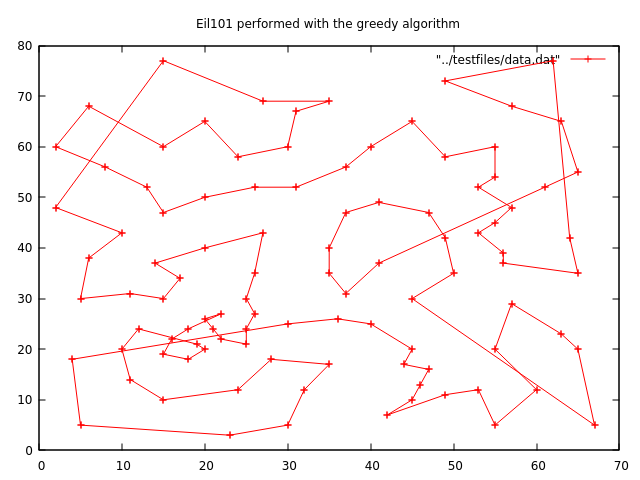
\includegraphics[width=0.6\textwidth]{images/eil101_greedy}
	\caption{In this figure we can see the application to eil101.tsp of the greedy algorithm. In particular we can see the long edges that are chosen since the procedure prefers the nodes that are close to each other.}
\end{figure}

\subsection{Extra-mileage algorithm}
This algorithm is more complex respect to the previous one but in favor of a better solution.

The idea in which the extra-mileage is the following: we start connecting the fartest nodes with both edges (like a cycle), than we search for the closest node to the edges, once it has been identified the edge is substitute with a new couple that insert the the node found in the solution. Let's explain it with the example shown in figure \ref{img:extra}.

\begin{figure}
	\centering
	\begin{subfigure}[b]{0.3\textwidth}
		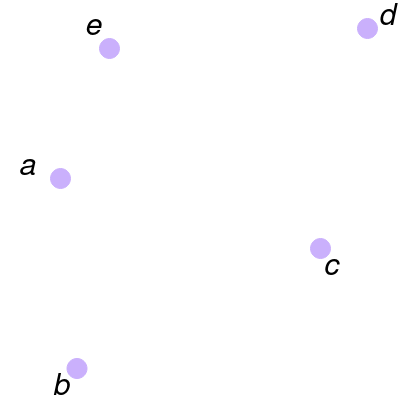
\includegraphics[width=\textwidth]{images/extra_1}
		\caption{No edges}
	\end{subfigure}
	\hfill
	\begin{subfigure}[b]{0.3\textwidth}
		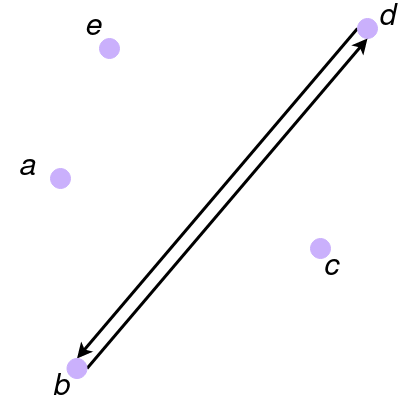
\includegraphics[width=\textwidth]{images/extra_2}
		\caption{First two edges added}
	\end{subfigure}
	\hfill
	\begin{subfigure}[b]{0.3\textwidth}
		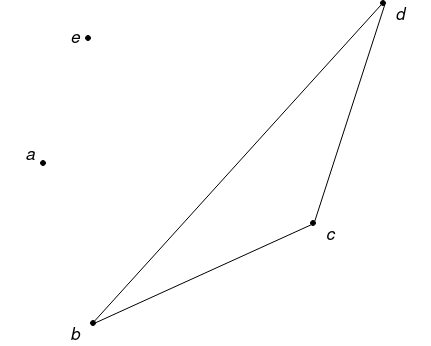
\includegraphics[width=\textwidth]{images/extra_3}
		\caption{One edge is substituted with other two connecting one more node}
	\end{subfigure}
	\bigskip
	\begin{subfigure}{0.3\textwidth}
		\centering
		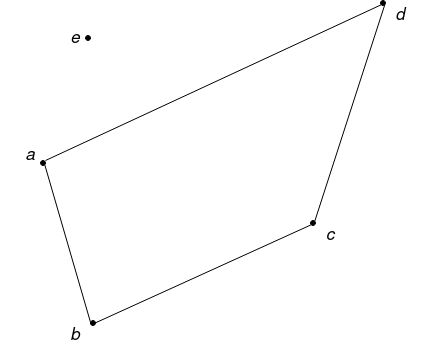
\includegraphics[width=\textwidth]{images/extra_4}
		\caption{Added one more node}
	\end{subfigure}
	\hfill
	\begin{subfigure}{0.3\textwidth}
		\centering
		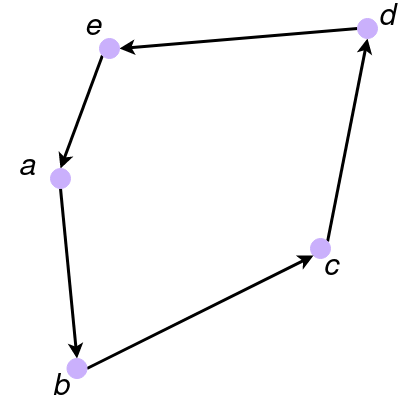
\includegraphics[width=\textwidth]{images/extra_5}
		\caption{All nodes are connected}
	\end{subfigure}
	\caption{In this image we can see the process done by extra-mileage to find the solution.}
	\label{img:extra}
\end{figure}

We start connecting with a cycle the fartest nodes (in this case $c$ and $d$), than we search the node that is closest to theese edges ($c$), once is found we substitute the edge with two more that allow the new node to enter the solution (in this case in order to allow $c$ to enter the solution one of the edges that connect $b$ and $c$ is removed and the edge $x_{bc}$ and $x_{cd}$ are added). This process is repeated until the solution is formed.

We can see the result of the algorithm in figure \ref{img:extra_sol}. Respect to the greedy algorithm we can see that is more ordered with less crossed edges.

\begin{figure}
	\centering
	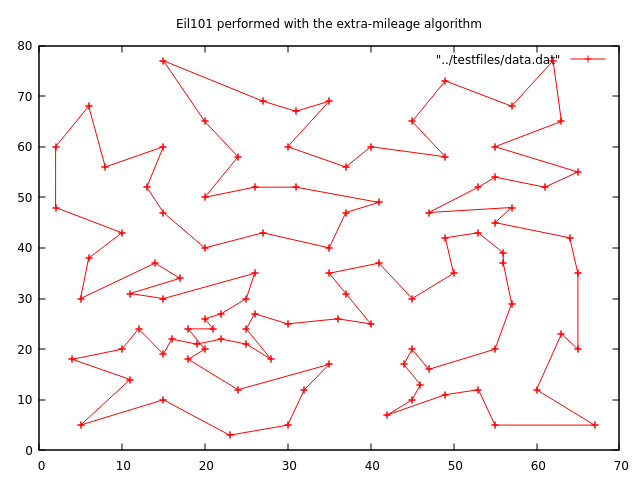
\includegraphics[width=0.6\textwidth]{images/eil101_extra_mileage}
	\caption{In this figure we can see the result of the application of the extra-mileage algortihm to eil101.tsp}
	\label{img:extra_sol}
\end{figure}

\subsection{k-\textit{opt} refining}
This section is not about an algorithm to solve the TSP problem but is about to refine (so improve) a solution that is already been found.\\
The process is based on the triangle inequality, in fact we are going to remove all the edges that cross each other. We can see an example of this operation in the image \ref{img:k_opt_example}, where the two edges that cross each other are sostitute by other to edges.

From a theoretical point of view the k-opt operation is a local search on the current solution, is not guaranteed to reach an optimal solution, but the objective value of the solution is going to always improve (if possible), in the worst case the solution will not change.

In our case we implemented two k-opt algorithms, the 2-opt and the 3-opt. We have decided to do that since as the $k$ grows the complexity grows with it. Just the implementation of the 3-opt algorithm is quite expensive from a computational point of view.

In the figure \ref{img:k_opt} we can see the differences between the 2-opt and 3-opt refining. In this images we applied theese algorithms starting from the solution provided by the greedy method to kroA200.tsp. \\
In the 2-opt application we started from a solution cost of $34543.0$ and than by the refining algorithm we reached the value $30189.0$ with a very little computational time, in fact it needed only $0.65$ seconds to reach the final solution.\\
In the 3-opt application we started from a solution cost of $34543.0$ and than by the refining algorithm we reached the value $25379.0$ in $77.37$ seconds.\\


\begin{figure}
	
	\centering
	\begin{subfigure}[b]{0.5\textwidth}
		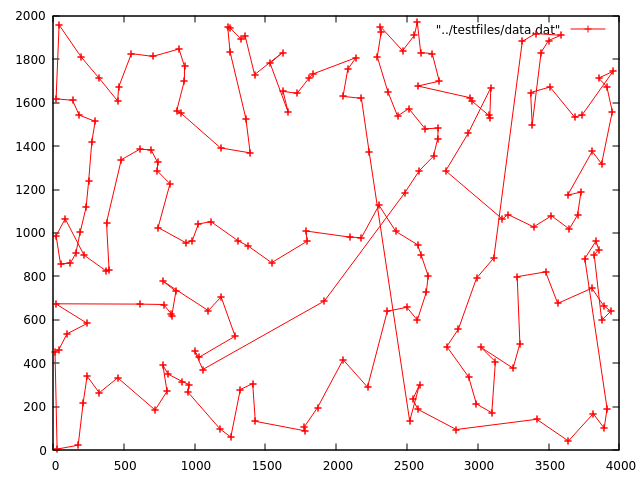
\includegraphics[width=\textwidth]{images/kroA_greedy}
		\caption{The instance kroA200.tsp solved with the greedy algorithm}
	\end{subfigure}
	\bigskip
	\begin{subfigure}[b]{0.5\textwidth}
		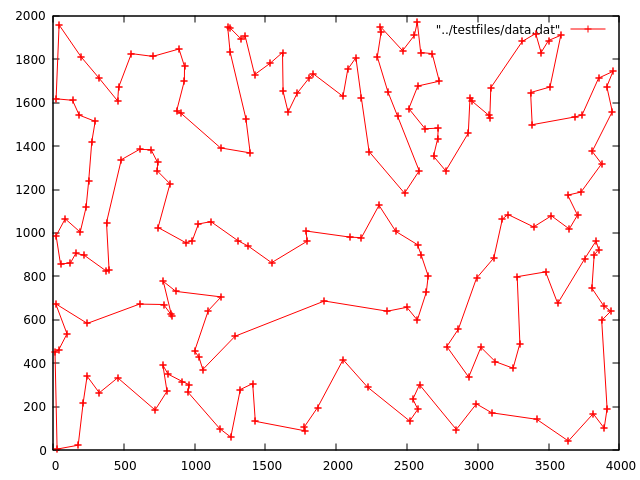
\includegraphics[width=\textwidth]{images/2_opt}
		\caption{Greedy + 2-opt refining}
	\end{subfigure}
	\bigskip
	\begin{subfigure}[b]{0.5\textwidth}
		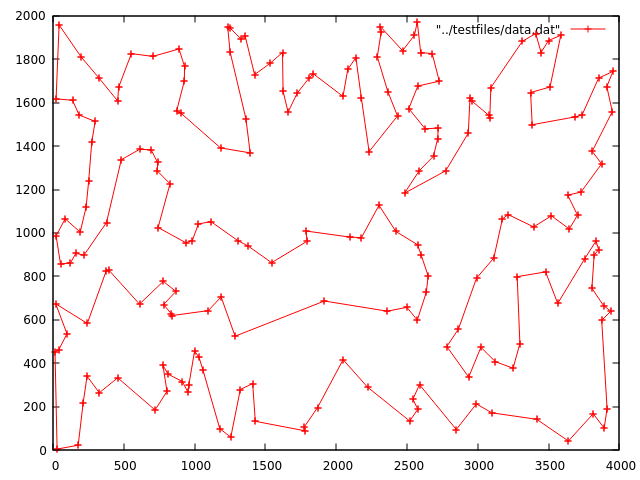
\includegraphics[width=\textwidth]{images/3_opt}
		\caption{Greedy + 3-opt refining}
	\end{subfigure}
	\caption{Comparison between the 2-opt and 3-opt refining}
	\label{img:k_opt}
\end{figure}

\subsection{Heuristics based on the branch and cut}
This section will explore the application of two heuristrics in the branch and cut method that we have seen in section \ref{sec:branch_and_cut}. Using these methods we can allow to the branch and cut method to solve even big instances but in a way that they probably never reach the optimal solution. The starting point of this section is basically the reduction of the search space.


\subsubsection{Hard-fixing}
The method of the hard-fixing expect to block the value of some variables in the problem in order to get the search space reduce in order to compute more easily a solution for it. The choice of which variable to block is due the user, but eventually can be completely random. 

The most important setting for this method is the starting solution, in fact since we are blocking the varibles so if the satarting solution is completely wrong the process of improving it will be more difficult. The process to retrieve a final solution is pretty easy: we start from that solution, we apply the branch and cut method for a predermined amount of time (or until it finds the optimal solution in the seach subspace), at the end of it we check if the new solution found is actually better than the previous one, if not we reduce the number of blocked variables and repeat the process. 

In our implementation we decided to put a percentage on the number of blocked variables, in particular we started from a value of $90\%$ and than for each time the solution found was not better than the previous one we reduced it by a $20\%$. The solution chosen as start was simply computed by the branch and cut method with the same time limit setted in the algorithm, in this way the starting point should never be a worse one.


\subsubsection{Soft-fixing}